%!TEX root = ../dokumentation.tex
\chapter{AR-Glass-Printer Implementierungen}
Im folgenden werden implemntierungsspezifische Details über das Unterstützten verschiedener AR-Geräte näher erläutert. Die mit einem AR-Gerät kommunizierenden Module sind hier als AR-Printer bezeichnet. 
Jeder AR-Printer ist für die Dauer einer Verbindung mit dem ihm zugeteilten Gerät umfassend verantwortlich für die Kommunikation zwischen App und Gerät.  Dies beinhaltet: 
\begin{enumerate}
	\item Den Verbindungsaufbau
	\item Die Verarbeitung von von der Applikation gesendeten Anfragen zur Textausgabe auf dem AR-Gerät
	\item Die Verarbeitung von vom AR-Gerät gesendeten Statusnachrichten\\
	\textit{Dies beinhaltet auch das Handling von Error-Codes.}
	\item Den Verbindungsabbau
\end{enumerate}
\par
Nachdem über das User Interface ein verfügbarer AR-Printer gewählt wurde, erzeugt eine Factory Klasse die jeweilige Printer-Instanz, welche im Konstruktor versucht eine Verbindung zum AR-Gerät aufzubauen. Ist der Verbindungsaufbau nicht möglich, wird der User über die fehlende Verbindung benachrichtigt und der Start-Record-Button deaktiviert, bis eine Verbindung zum Gerät hergestellt wurde oder vom User ein anderer AR-Printer gewählt wird.

\section{Die Klasse AbstractPrinter}
Die Klasse AbstractPrinter implementiert das Interface IPrinter und abstrahiert gemeinsames Verhalten aller AR-Printer. Die Implementierung eines spezifischen AR-Printers erfolgt über die Ableitung dieser Klasse und nicht über das Interface direkt. Dies dient der Vermeidung von Fehlern und der Vereinheitlichung der Arbeitsweise von unterschiedlichen Implementierungen.\\
\paragraph{Implementierte Methoden}
Während der Verbindungsauf- beziehungsweise -abbau geräte- und somit implementierungsspezifisch sind, kann das Verhalten der Methoden startPrinting(), addToMessageBuffer(String message),  und stopPrinting() Geräteübergreifend implementiert werden.\\
Die Methode addToMessageBuffer(String message) erfüllt die Aufgabe, den übergebenen String zum Message Buffer hinzuzufügen. Der Message Buffer ist durch eine LinkedBlockingQueue realisiert und stellt somit eine Schlange dar, bei der Entnahmen immer am vorderen Ende geschehen und Elemente an ihrem Ende angefügt werden können. Sie arbeitet nach dem First-In-First-Out-Prinzip.\\
Die Methode startPrinting() erzeugt einen neuen Thread, welcher innerhalb einer eigenen Methode doPrinterJob() eine Schleife solange durchläuft, bis das boolsche Attribut isProcessing auf false gesetzt wurde, was bei Beendigung des Konvertierungsvorgangs der Fall ist.
Innerhalb der Schleife wird überprüft, ob der Message Buffer neue Elemente zur Entnahme enthält. Ist dies der Fall, wird erfolgt ein Aufruf der abstrakten Methode printMessage(String message), welche die Nachricht im gerätespezifischen Protokol an das verbundene AR-Gerät sendet. Diese Methode muss für jeden spezifischen AR-Printer implementier eigens implementiert werden. Ein boolscher Rückgabewert gibt Auskunft über den Erfolg des Sendens der Nachricht. Liefert die Überprüfung der isProcessing-Variable false zurück, so deutet dies auf das Ende des Vorgangs hin. Um Ausgaben nicht apprupt zu beenden, wird neben des isProcessing-Attributes auch noch der Inhalt des Message Buffers geprüft. Is isProcessing zwar false, aber der Message Buffer enthält noch Elemente, die zur Ausgabe in Auftrag gegeben wurden, fährt der Printing-Thread fort, bis alle Ausgaben getätigt wurde.\\
Die Methode stopPrinting() setzt das boolsche Attribut isProcessing auf false. Dies führt zum Beenden der Schleife innerhalb des Printing-Threads und somit zur Beendigung des Threads an sich.
\section{Support der GlassUp AR Brille}
\begin{figure}{l}{1\linewidth}
	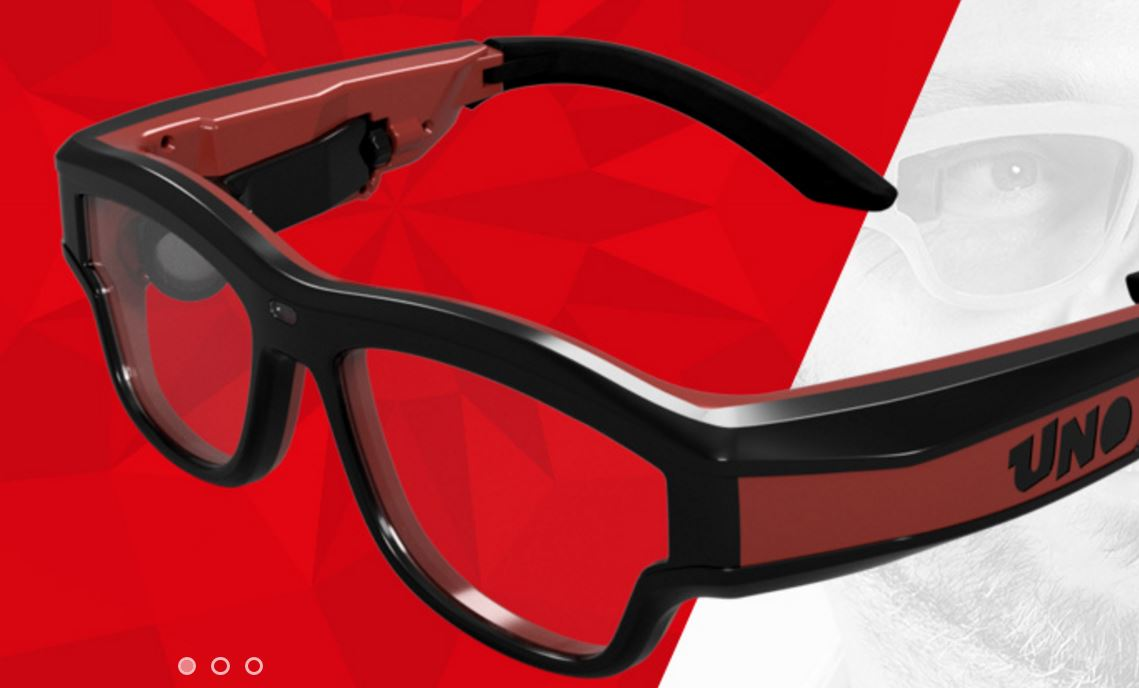
\includegraphics[width=\linewidth]{../images/glassUpGlasses.jpg}
	\caption{Die GlassUp Augmented Reality Brille\cite{home}}
	\label{fig:GlassUpGlasses}
\end{figure}
\paragraph{Die GlassUp Brille}
GlassUp ist ein italienisches Unternehmen, welches eine 65 Gramm \cite{faq} schwere Augmented Reality Brille herstellt. Sie ist in \ref{fig:GlassUpGlasses} abgebildet. Die Brille befindet sich zwar noch in der Entwicklung, kann aber alles bieten, was zur Funktionalität unserer Applikation notwendig ist:\\
Nach eigener Aussage legt die Firma Wert darauf, eine unauffällige Brille zu produzieren, welche weniger einen Multimedialen Gegenstand als einen generellen Alltagshelfer darstellt \cite{home}.\\
So besitzt diese Brille keine Kamera, wie beispielsweise die von Google angebotene Alternative\cite{google glasses}. Eine Kamera gefährdet den Einsatz der Augmented Reality Brille insoweit, dass nach Paragraph 90 des Telekommunikationsgesetzes der Besitz von Gegenständen, "die ihrer Form nach einen anderen Gegenstand vortäuschen oder die mit Gegenständen des täglichen Gebrauchs verkleidet sind und auf Grund dieser Umstände [...] dazu bestimmt sind, das [...] Bild eines anderen von diesem unbemerkt aufzunehmen."\\
Auch ist die GlassUp Brille mit einem Preis von 299 Euro \cite{faq} noch erschwinglich. Die frei erhältliche SDK enthält außerdem einen Emulator, wodurch ein Brillenkauf für Entwicklungszwecke nicht von Anfang an zwangsläufig notwendig ist \cite{SDK}.\\
Die Brille wird durch die Bluetooth-Technik mit einem Mobiltelephon verbunden und Projeziert Texte und einfache Grafiken in der Farbe grün in den Mittelpunkt des Sichtfelds des Anwenders.
Sie verfügt über ein Touchpad mit drei Eingabeknöpfen, durch die Smartphone-Anwendungen alternativ gesteuert werden können.
Der niedrige Preis, sowie der kompakte aber ausreichende Funktionsumfang führten zur Entscheidung, diese Brille als erste zu Unterstützen. Erweiterungen zum Unterstützen weiterer Brillen, sind durch den modularen Aufbau der Applikation allerdings ohne weiteres möglich.

\paragraph{Der GlassUp-Connector}





 \begin{lstlisting}
[caption={Die Methode addMessageToLineList(String Message) der Klasse GlassUpPrinter}\label{lst:GlassUpPrinter: addMessageToLineList(String message)},captionpos=t] 
/**
* method takes a message and splits it in lines of 16 chars
* to be printed to the AR device. The lines are added to this.linesToPrint
* @param messageBuffer
*/
private boolean addMessageToLineList(String messageBuffer){
int counter = 0;

if(messageBuffer == null){
return false;
}

while(counter < messageBuffer.length()) {

if (messageBuffer.length() - (counter + 17) <= 0) {
//rest of buffer is smaller than one line, -> prepare buffer and send
//then break
this.linesToPrint.add(messageBuffer.substring(counter));
break;
}
//after 17 signs there is a space --> perfect line
if (messageBuffer.charAt(counter + 17) == ' ') {
this.linesToPrint.add(messageBuffer.substring(counter, counter + 18));
counter += 18;
} else {
//check next ' ' before 17
boolean foundSpace = false;

for (int i = counter + 17; i > counter; i--) {
//space found?
if (messageBuffer.charAt(i) == ' ') {
this.linesToPrint.add(messageBuffer.substring(counter, i+1));
counter = i + 1;
foundSpace = true;
break;
}
}

//check if a space was found in the line
if (!foundSpace) {
//if no space in whole line just break on letter 17
this.linesToPrint.add(messageBuffer.substring(counter, counter+17));
counter += 17;
}
}
}
return true;
}
\end{lstlisting}
%Algorithmus zur formatierung
\section{Der TextField Printer}